%\part{Introduction}
\chapter{Introduction}
\label{chap: Chapter 1}

Academic content generation has seen an increase in recent years. Getting usable research papers has become a problem. In order to produce reputable and quality papers, vast amounts of research need to be consulted in several domains and sub-domains. Reading and working through the additional research papers can be time consuming and could result in researchers overlooking important topics and discussions.

This study is a exploratory study into how machine learning (ML) coupled with natural language processing can aid in identifying usable research papers with less effort. However, it quickly became clear that machine learning and natural language processing is rich in aiding techniques and algorithms.

This chapter sets the groundwork of the research project. The problem area consists of a brief introduction into machine learning, topic modeling and clustering techniques, leading to the problem statement. In addition, research objectives are identified. Thereafter, the research process is described which was followed to achieve the research objectives. The chapter ends with the chapter outline for the rest of the dissertation and a brief conclusion to the chapter.


\section{Background}

Information overload is a real phenomenon in our digital age, and our access to knowledge and resources have exceeded our capacity to comprehend. The emergence of online databases has made the ability to search, find, retrieve and summarise documents increasingly difficult. The possibilities have increased drastically in recent years of using machine learning (ML), information retrieval (IR) and natural language processing (NLP) to ease this immense task of navigating through the same databases.

\citeA{Andriybook2019} describes machine learning as a subfield of computer science, which uses algorithms to help identify certain objectives. There are three paradigms of machine learning:

\begin{enumerate}
    \item Reinforcement learning – primarily focuses on training machine learning models to perform a sequence of decisions based on data \cite{DBLP:journals/corr/abs-1806-08894}.
    \item Supervised learning – is a machine learning task that maps input to output based on tagged or labelled datasets \cite{singh2019natural}.
    \item Unsupervised learning – is defined as mapping inputs to outputs but the datasets do not contain any tagging or labels \cite{hastie2009unsupervised}.
\end{enumerate}

Information retrieval is a mixture of information systems, databases and data mining techniques \cite{baeza1999modern}. Furthermore, \citeA{baeza1999modern} mentioned that information retrieval includes techniques which aid searching for information in a document. Another technique, called text mining, also intersects information retrieval and machine learning.

The text mining approach seeks to identify words and phrases that could explain certain underlying structure in the data. Text mining has focused on analysing co-occurrence data through association rules, distribution analysis, and different clustering approaches. Utilising these approaches to create practical categories rather than using predefined categories, opens up a world of new research options. \citeA{hofmann2017probabilistic} suggests that topic modeling would be a useful tool to extract information from textual data.

\section{Description of Problem Area} \label{ssec:prob}

As mentioned in the previous section, information overload has become a real problem in recent years. More specifically, researchers have indicated that information overload has caused three main difficulties \cite{al2021exploring}. They are; difficulty to process the information which was collected, difficulty to find relevant and quality information and lastly, there are just too much information generated.

Researchers experience difficulty when seeking information they develop cognitive barriers \cite{savolainen2015cognitive}. Five sub-types of cognitive barriers are reported by the study: (1) not able to differentiate between the information needs and the research needs, (2) inability to formulate information needs, (3) not aware of the various information sources, (4) low self-efficacy, and (5) unable to deal with information overload.

The best way to combat information overload from an personal and technological perspective, is better designed information systems. Such information systems will enable the researcher to better balance the scale between consuming information and understanding it \cite{bawden2020information}.



As mentioned in the previous section, information overload has become a real problem in recent years. More specifically, researchers have indicated that information overload has caused three main difficulties \cite{al2021exploring}. They are: difficulty to process the information which was collected; difficulty to find relevant and quality information; and lastly, there is just too much information generated.

Researchers experiencing difficulty when seeking information develop cognitive barriers \cite{savolainen2015cognitive}. Five sub-types of cognitive barriers are reported by the study: (1) not being able to differentiate between information needs and research needs, (2) inability to formulate information needs, (3) not being aware of the various information sources, (4) low self-efficacy, and (5) inability to deal with information overload.

The best way to combat information overload from both a personal and a technological perspective, is to have better designed information systems. Such information systems will enable the researcher to balance the scale better between consuming information and understanding it \cite{bawden2020information}.

This leads to the following problem statement:

\textbf{\textit{To identify related research papers is a time consuming cognitive barrier.}}

\section{Research Objective} \label{ssec: Chapter 1}

Research objectives are derived from the problem statement. In order to satisfy the problem described above, the primarily research objective is to:

\textbf{\textit{Develop a model to recommend related research papers}}

This model is to be developed with the intention of aiding academics in any research field. For this to be achieved, the following sub-objectives must be achieved:
\begin{itemize}
  \item[SO1:] To identify recommender systems techniques and how they are used.
  \item[SO2:] To identify machine learning techniques that assist with the recommender task.
\end{itemize}

The model will include recommender system- and machine learning techniques. The development of the prototype is to show that the model is feasible to implement. Furthermore, it serves to demonstrate applicability by using information security South Africa data. Throughout the development of the model and prototype practical lessons were learned, which will be discussed in Chapter \ref{chap: Chapter 7}.

In the next section, the research process will be discussed.

\section{Research process}

Owing to the fact that this research study is primarily experimental in nature, a model and a prototype were developed. A broader explanation of the paradigm, the research position itself, and also which methods were used throughout the study, are presented in Chapter \ref{chap: Chapter 4}.

\section{Delineation}

This study included the development of a prototype that was built using text mining and natural processing techniques. Furthermore, the techniques used were not chosen based on experimentation but were derived from literature. 
The prototype was developed to only identify topics and needs a certain level of manual intervention to validate the recommendations.
The prototype was done in the Python 3 environment and used several NTLK and Gensim libraries. The dataset was obtained and used which was made available on the Information Security South Africa website. 


\section{Ethical Consideration}

No ethical clearance was needed to complete this study. All of the data was used from a publicly available source and do not contain personal or sensitive data. No human interaction was needed to complete this study.

\section{Chapter Outline}
Figure \ref{fig:Dlayout} provides the layout of this dissertation. It can be categorised into three parts: 
\textit{Introduction, prototype development, and lessons learned and conclusion.}

The \textit{Introduction} part includes Chapter \ref{chap: Chapter 1} to \ref{chap: Chapter 3}.
Chapter \ref{chap: Chapter 1} provides the introduction and background to this study. This is followed by the problem statement and the objectives. Lastly, it refers to the research process, which will be discussed in Chapter \ref{chap: Chapter 4}. Chapter \ref{chap: Chapter 2} focuses on recommender systems and what constitutes a recommendation task. Furthermore, it discusses each recommender system method, along with examples of each. Chapter \ref{chap: Chapter 3} investigates the various machine learning technologies that were considered in this study. Chapter \ref{chap: Chapter 3} concludes by investigating document clustering and which techniques should be used.

The \textit{model development} part includes Chapters \ref{chap: Chapter 4} to \ref{chap: Chapter 6}. Chapter \ref{chap: Chapter 4} focuses on the research process which was followed in this study, highlighting the research methods used. Chapter \ref{chap: Chapter 5} deals with the development of the model derived from the research design chapter. Chapter \ref{chap: Chapter 6} outlines the techniques and methods that were used in the development. 

As seen in Figure \ref{fig:Dlayout}, Chapter \ref{chap: Chapter 6} is created with a dual purpose: (1) while developing the prototype, certain parameters were identified which influenced the quality of the prototype and model, (2) using recommender system concepts, machine learning algorithms and data from an information security conference showed that the model was applicable and feasible.

The \textit{lessons learned and conclusion} part includes Chapter \ref{chap: Chapter 7} and Chapter \ref{chap: Chapter 8}. 
Chapter \ref{chap: Chapter 7} focuses on practical lessons learned during the development of the model and prototype. Chapter \ref{chap: Chapter 8} concludes the study by summarising it and revisits the research objectives and hints to further research to be done.


The \textit{lessons learned and conclusion} part includes Chapter \ref{chap: Chapter 7} and Chapter \ref{chap: Chapter 8}. Chapter \ref{chap: Chapter 8} focuses on practical lessons learned during the development of the model and prototype. Chapter \ref{chap: Chapter 8} concludes the study by summarising it. It revisits the research objectives and hints at further research to be done.

\begin{figure}[htbp]
\centering
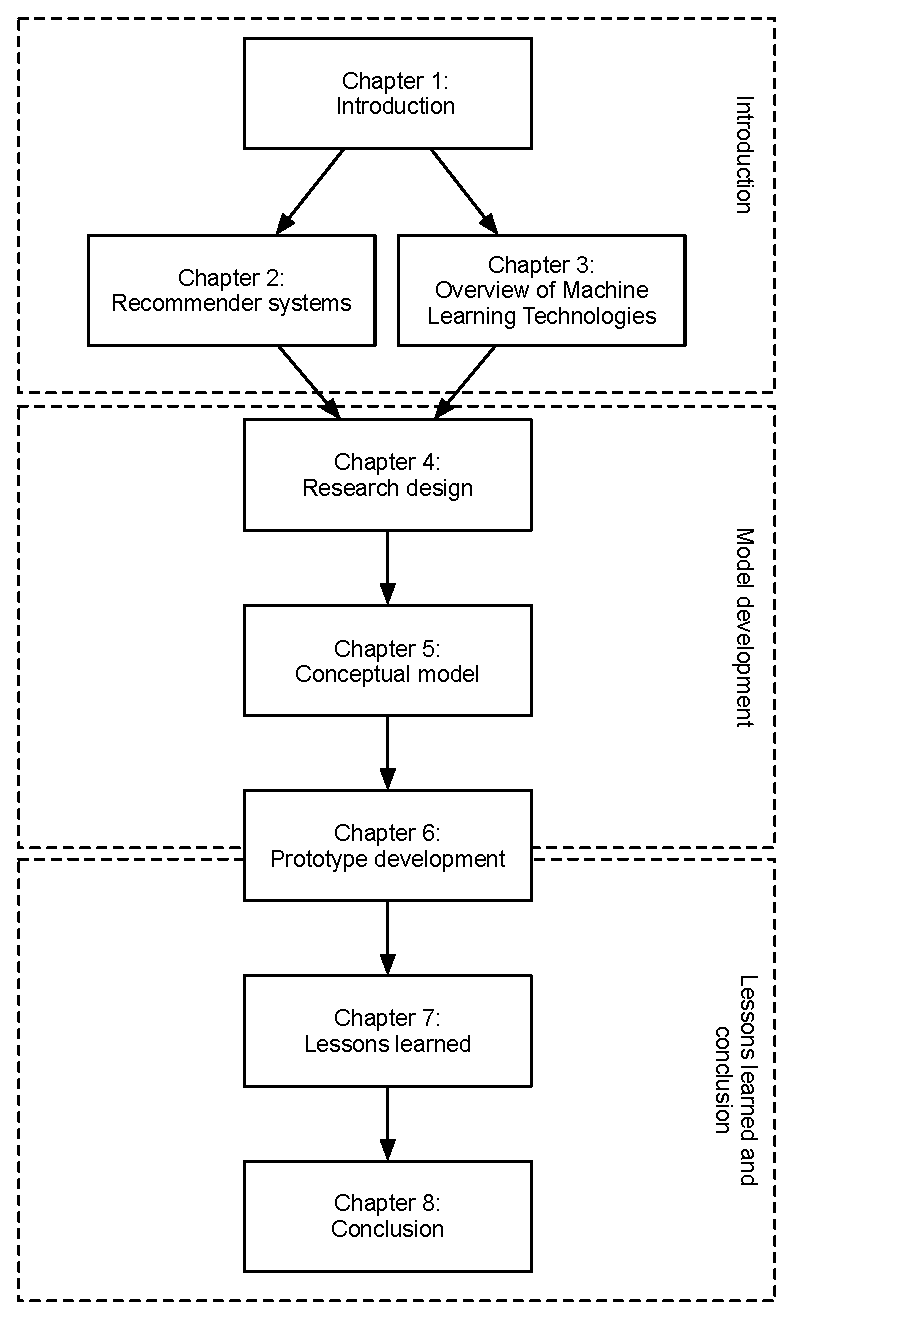
\includegraphics[width=10cm]{./figures/overlast222.eps}
\caption{Layout of the Dissertation}
\label{fig:Dlayout}
\end{figure}
